\documentclass[a4paper, 11pt, notitlepage]{article}

%\usepackage{babel}
\usepackage[utf8]{inputenc}
\usepackage[T1]{fontenc, url}
\usepackage{textcomp}
\usepackage{amsmath, amssymb}
\usepackage{amsbsy, amsfonts}
\usepackage{graphicx, color}
\usepackage{parskip}
\usepackage{framed}
\usepackage{amsmath}
\usepackage{xcolor}
\usepackage{multicol}
\usepackage{url}
\usepackage{flafter}
\usepackage{caption}

%\DeclareCaptionLabelSeparator{colon}{. }
\renewcommand{\captionfont}{\sffamily}
\renewcommand{\captionlabelfont}{\bf\sffamily}
\setlength{\captionmargin}{40pt}

\usepackage{geometry}
\geometry{headheight=0.01mm}
\geometry{top=24mm, bottom=29mm, left=39mm, right=39mm}

\renewcommand{\arraystretch}{2}
\setlength{\tabcolsep}{10pt}
\makeatletter
\renewcommand*\env@matrix[1][*\c@MaxMatrixCols c]{%
  \hskip -\arraycolsep
  \let\@ifnextchar\new@ifnextchar
  \array{#1}}
%
% Parametere for inkludering av kode fra fil
%
\usepackage{listings}

\DeclareMathAlphabet{\mathbfit}{OML}{cmm}{b}{it}

\definecolor{javared}{rgb}{0.6,0,0} % for strings
\definecolor{javagreen}{rgb}{0.25,0.5,0.35} % comments
\definecolor{javapurple}{rgb}{0.5,0,0.35} % keywords
\definecolor{javadocblue}{rgb}{0.25,0.35,0.75} % javadoc

\lstset{language=python,
basicstyle=\ttfamily\scriptsize,
keywordstyle=\color{javapurple},%\bfseries,
stringstyle=\color{javared},
commentstyle=\color{javagreen},
morecomment=[s][\color{javadocblue}]{/**}{*/},
% numbers=left,
% numberstyle=\tiny\color{black},
stepnumber=2,
numbersep=10pt,
tabsize=4,
showspaces=false,
captionpos=b,
showstringspaces=false,
frame= single,
breaklines=true}
%
% Definering av egne kommandoer og miljøer
%
\newcommand{\dd}[1]{\ \text{d}#1}
\newcommand{\f}[2]{\frac{#1}{#2}} 
\newcommand{\beq}{\begin{equation}}
\newcommand{\eeq}{\end{equation}}
\newcommand{\bra}[1]{\langle #1|}
\newcommand{\ket}[1]{|#1 \rangle}
\newcommand{\braket}[2]{\langle #1 | #2 \rangle}
\newcommand{\braup}[1]{\langle #1 \left|\uparrow\rangle\right.}
\newcommand{\bradown}[1]{\langle #1 \left|\downarrow\rangle\right.}
\newcommand{\av}[1]{\left| #1 \right|}
\newcommand{\op}[1]{\hat{#1}}
\newcommand{\braopket}[3]{\langle #1 | {#2} | #3 \rangle}
\newcommand{\ketbra}[2]{\ket{#1}\bra{#2}}
\newcommand{\pp}[1]{\frac{\partial}{\partial #1}}
\newcommand{\ppn}[1]{\frac{\partial^2}{\partial #1^2}}
\newcommand{\up}{\left|\uparrow\rangle\right.}
\newcommand{\upup}{\left|\uparrow\uparrow\rangle\right.}
\newcommand{\down}{\left|\downarrow\rangle\right.}
\newcommand{\downdown}{\left|\downarrow\downarrow\rangle\right.}
\newcommand{\updown}{\left|\uparrow\downarrow\rangle\right.}
\newcommand{\downup}{\left|\downarrow\uparrow\rangle\right.}
\newcommand{\bupup}{\left.\langle\uparrow\uparrow\right|}
\newcommand{\bdowndown}{\left.\langle\downarrow\downarrow\right|}
\newcommand{\bupdown}{\left.\langle\uparrow\downarrow\right|}
\newcommand{\bdownup}{\left.\langle\downarrow\uparrow\right|}
\renewcommand{\d}{{\rm d}}
\newcommand{\Res}[2]{{\rm Res}(#1;#2)}
\newcommand{\To}{\quad\Rightarrow\quad}
\newcommand{\eps}{\epsilon}
\newcommand{\inner}[2]{\langle #1 , #2 \rangle}


\newcommand{\bt}[1]{\boldsymbol{#1}}
\newcommand{\mat}[1]{\textsf{\textbf{#1}}}
\newcommand{\I}{\boldsymbol{\mathcal{I}}}
\newcommand{\p}{\partial}
%
% Navn og tittel
%
\author{Jonas van den Brink \\[-0.2cm] \texttt{j.v.d.brink@fys.uio.no}}
\title{Battleship! \\ Avsluttende prosjekt i programmeringskurs \\ Bjørnegård Skole}

\begin{document}

\maketitle

\thispagestyle{empty}

Vi har nå kommet til siste uke av kurset, og dere har sett en del Python kode og fått prøvd dere mye selv. Vi skal nå igang med siste del av kurset, der dere selv skal kode en versjon av brettspillet \emph{Battleship!}. Mye av disse oppgaven er hentet fra Code Academy, du kan også løse dem der ved å gå inn på denne lenken og lete deg frem til riktig modul

\begin{center}
\url{http://www.codecademy.com/en/tracks/python}
\end{center}

\subsection*{Hva er Battleship?}

Battleship er et brettspill for to personer. Begge spillerene får utdelt et visst antall skip som de må plassere på et rutenett. Etter begge spillerene har plassert ut alle skipene sine, så gjetter de annenhver gang på koordinatene til mostanderens skip. Etter de gjetter på koordinatene, så svarer motstanderen om det var et treff eller et bom. Spillerene har to brett, et til å holde styr på sine egne skip og et til å holde styr på hvor de har skutt. På figuren under ser du spillbrettet. De hvite pinsene viser skudd som har bommet, og de røde viser skudd som har truffet.

\begin{center}
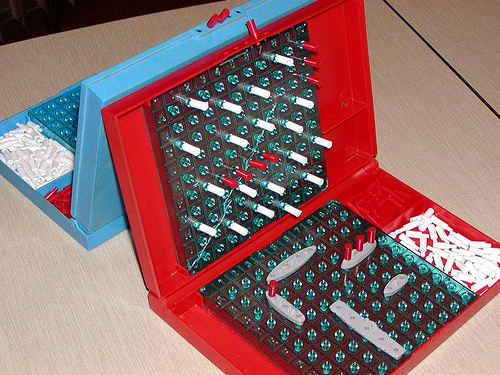
\includegraphics[width=0.6\textwidth]{battleship-board-game}
\end{center}

\subsection*{Hva vi skal gjøre i dette prosjektet.}

Dette spillet kan dere lage på datamaskin ved hjelp av den programmeringen dere har lært i dette kurset, men vi har litt begrenset tid - så vi skal lage en litt forenklet versjon. For det første holder vi oss til `single-player', vi starter også med et litt mindre spillbrett og færre skip. Etter du har fått laget et forenklet spill som fungerer bra, så kan du utvide det litt og litt til du har et stort og bra spill! Vi får se hvor langt vi kommer iløpet av denne økten.

\section*{La oss sette igang!}

\subsection*{Lage spillbrettet}
Det første vi må gjøre er å lage selve spillbrettet. Spillbrettet representerer havet og det skal være et rutenett slik at vi kan gjette på en rute ved å gi de to koordinatene, $x$ og $y$. La oss lage et brett som er 5x5. Hvis vi tegner det for hånd, så hadde det sett sånn her ut:

\begin{center}
\begin{tabular}{|c|c|c|c|c|}
\hline 
O & O & O & O & O \\ \hline
O & O & O & O & O \\ \hline
O & O & O & O & O \\ \hline
O & O & O & O & O \\ \hline
O & O & O & O & O \\ \hline
\end{tabular}
\end{center}

Du kan lage denne på datamaskin ved å bruke en liste med lister. Hvis vi lar en liste bestå av 5 elementer, der hvert element er en liste med 5 elementer som bare er ``O'' (Stor o, ikke null), så vil det være spillbrettet vårt.

\subsubsection*{Oppgaver}
\begin{itemize}
	\item[(a)] Lag en variabel, \verb+board+, som er en tom liste.
	\item[(b)] Legg listen \verb+["O", "O", "O", "O", "O"]+ til \verb+board+ fem ganger. \\ \textbf{Hint: board.append(...)}.
	\item[(c)] Skriv ut \verb+board+ og se at du har fått totalt 25 ganger ``O''.
\end{itemize}

Når du skriver ut \verb+board+, så blir ikke utskriften et fint rutenett sånn som vi tegnet for hånd. La oss fikse dette. Vi kommer til å ha lyst til å skrive ut spillbrettet vårt flere ganger iløpet av spillet, så vi har lyst til å lage en funksjon som gjør dette for oss. Vi kan starte å lage en funksjon som dette
\begin{lstlisting}
def print_board(board):
	...
\end{lstlisting}
Husk innrykket! Inne i funksjonen har vi lyst til å ha en løkke som går gjennom \verb+board+-lista og skriver hver rad av spillbrettet på en egen linje.
\begin{lstlisting}
for row in board:
	print row
\end{lstlisting}

\subsubsection*{Oppgaver}
\begin{itemize}
	\item[(d)] Lag funksjonen \verb+print_board+ ved å fylle inn for `...'
	\item[(e)] Sjekk at funksjonen fungerer ved å kalle på den med \verb+print_board(board)+. 
	\item[(f)] Istedenfor å bare skrive \verb+print row+ inne i for-løkka, kan du skrive \\[0.2cm] \verb+print " ".join(row)+ \\[0.2cm]
	 Da blir utskriften enda finere.
\end{itemize}
Før du går videre bør du få en utskrift som er et fint rutenett, hvis du ikke får til det er det på tide å få litt hjelp, enten fra sidemannen eller fra oss.

Nå som du har laget spillbrettet vi skal bruke og du kan skrive det ut pent, må du forstå hvordan vi kan endre på spillbrettet. Jeg minner nå om at vi endrer på en liste ved hjelp av \emph{indeksering}. Hvis vi har en enkel liste
\begin{lstlisting}
names = ["Lisa", "Mary", "Marcus"]
\end{lstlisting}
så kan vi for eksempel endre `Marcus' til `Markus' ved å skrive
\begin{lstlisting}
names[2] = "Markus"
\end{lstlisting}
Husk at python begynner å telle på 0!

Siden spillbrettet vårt består av lister inne i lister, så vil for eksempel \verb+board[0]+ være listen \verb+["O", "O", "O", "O", "O"]+ som vi da kan indeksere på nytt! Altså kan vi gjøre for eksempel dette 
\begin{lstlisting}
board[0][0] = "X"
\end{lstlisting}
Vi har nå endret koordinat (0, 0) på spillbrettet vårt til å være `X', istedenfor `O'. Prøv deg litt frem til du har god forståelse av hvordan det fungerer
\subsubsection*{Oppgaver}
\begin{itemize}
	\item[(g)] Kjør kommandoen \verb+board[0][0] = "X"+ og bruk deretter \verb+print_board(board)+ for å se resultatet. Hvilket element endret vi på?
	\item[(h)] Endre feltet i midten av spillbrettet til å være `X'.
\end{itemize}

Nå har vi altså laget spillbrettet vårt, laget en funksjon \verb+print_board+ som skriver det ut som et fint rutenett og vi har funnet ut hvordan vi kan gå inn og endre det. La oss nå se på hvordan vi kan plassere ut og skyte på skipene.

\clearpage

\section*{Plassere ut skip}

La oss starte med å plassere ut et fiendtlig skip som bare dekker 1 enkelt rute til å begynne med. Skipet skal kunne være hvor som helst på hele kartet. Siden kartet vårt er et 5x5 rutenett, kan vi si at ruten skipet er i vil ha en $x$ og en $y$-koordinat som går fra 0 til 4. 

Det skal være tilfeldig hvor skipet er hver gang spillet spilles. Du kan få til å plassere skipet tilfeldig ved å trekke koordinatene tilfeldig.

\subsubsection*{Oppgaver}
\begin{itemize}
	\item[(i)] Importer funksjonen \verb+randint+ fra random. 
	\item[(j)] Lag en variabel \verb+ship_x+ og sett den lik et tilfeldig tall mellom 0 og 4.
	\item[(k)] Lag en variabel \verb+ship_y+ og sett den lik et tilfeldig tall mellom 0 og 4.
\end{itemize}

Vi har nå trukket koordinatene til skipet tilfeldig og lagret dem i variabelene \verb+ship_x+ og \verb+ship_y+. For koden vi skal skrive videre er det nyttig å vite akkurat hvor skipet befinner seg, sånn at vi kan teste programmet vårt lettere. Du kan finne ut hvor skipet er rett og slett ved enten å skrive ut koordinatene
\begin{lstlisting}
print ship_x
print ship_y
\end{lstlisting}
eller du kan endre spillbrettet så man ser det når man skriver ut brettet
\begin{lstlisting}
board[ship_x][ship_y] = "+"
print_board(board)
\end{lstlisting}

Uansett hvilken av disse løsningene du går for, er det viktig at du husker å fjerne utskriften når du har skrevet og testet ferdig programmet ditt, ellers blir spillet altfor lett for den som spiller det.

\subsection*{Skyte på skipet!}

Vi er nå klare for å få brukeren til å prøve å skyte ned skipet, da må vi få brukeren til å gjette på hvor skipet er. Forhåpentligvis er du vant med hvordan du stiller brukeren spørsmål, det gjør du med \verb+raw_input()+.
\begin{itemize}
	\item[(l)] Lag en variabel \verb+guess_x+ og bruk \verb+raw_input()+ til å lagre svaret fra brukeren.
	\item[(l)] Funksjonen \verb+raw_input()+ vil alltid lage tekststrenger, men vi vil at \verb+guess_x+ skal være et heltall. Gjør slik at \verb+guess_x+ er et heltall. \\ 
			   \textbf{Hint: } \verb+guess_x = int(raw_input(...))+
	\item[(m)] Lag en variabel \verb+guess_y+ og gjør tilsvarende som for x-koordinaten.
\end{itemize}

\clearpage

Nå som vi har trukket posisjonen til skipet tilfeldig, og vi har spurt brukeren hvor de har lyst til å skyte, så er vi klare til å sjekke om brukeren traff. Dette gjør vi selvsagt med en \verb+if+-test. I første omgang er det bare to muligheter, enten traff brukeren, eller så bommet hun. For at det skal være et treff, så må selvfølgelig begge koordinatene stemme! Altså må \verb+ship_x+ og \verb+guess_x+ være like \textbf{og} \verb+ship_y+ og \verb+guess_y+ være like.
\begin{itemize}
	\item[(n)] Skriv en \verb+if+-test som sjekker om \verb+ship_x == guess_x+ og \verb+ship_y == guess_y+. Hvis det er tilfellet, skriv ut en beskjed om at brukeren traff. 
	\item[(o)] Legg til en \verb+else+-blokk der du skriver ut en beskjed om at brukeren bommet.
	\item[(p)] Test programmet ditt, der du med vilje treffer. Prøv så med en bom. Fungerer alt som forventet?
\end{itemize}

I tilegg til å bare skrive ut en beskjed dersom brukeren gjetter feil, bør vi endre spillbrettet så brukeren kan se hvor de allerede har skutt. La oss bruke `X' for å vise at et felt har blitt skutt på men var et bom.

\begin{itemize}
	\item[(q)] I \verb+else+-blokken din, endre feltet i spillbrettet som har koordinater \verb+guess_x+ og \verb+guess_y+ til \verb+"X"+. Skriv også ut brettet \\
	\textbf{Hint:} \begin{lstlisting}
		if ...:
			print ...
		else:
			print ...
			board[...][...] = ...
			print_board(board)
	\end{lstlisting}
	\item[(p)] Test programmet ditt med en bom for å se at det fungerer som det skal.
\end{itemize}

\subsection*{Flere skudd}

Hitil har brukeren bare fått lov til å prøve å skyte ned skipet 1 gang, det er litt lite! Vi skal nå bruke en løkke sånn at brukeren kan skyte opp til 10 ganger! Vi velger å bruke en \verb+while+-løkke som gjentar seg helt til brukeren har enten vunnet, eller bommet 10 ganger. Vi må da holde styr på hvor mange ganger brukeren har bommet.

\begin{itemize}
	\item[(r)] Lag en variabel \verb+misses+ og sett den til å være 0.
	\item[(s)] Gi all kode som skal gjenta seg selv et innrykk, du gjør dette enkelt ved å merke alle linjer som skal ha innrykk samtidig og trykke på tab-knappen. \\ \textbf{Hint: } Det vi vil at skal gjenta seg selv, er at brukeren gjetter på koordinater, og så at vi sjekker gjettene og oppdaterer brettet
	\item[(t)] Rett før kodeblokken du nettopp ga innrykk, start \verb+while+-løkken din. \\ 
	\textbf{Hint:} \verb+ while misses ... :+
	\item[(u)] Inne i løkka di må du huske på å øke variabelen \verb+misses+ når brukeren bommer. Oppdater programmet ditt slik at den teller opp hver gang brukeren bommer.  \\ \textbf{Hint: } \verb!misses += 1!
	\item[(v)] På starten av løkka di, før du spør brukeren om å gjette. Skriv ut en beskjed som forteller hvor mange skudd de har igjen.
	\item[(w)] Test programmet ditt og sjekk at løkka fungerer som den skal.
\end{itemize}

En ting som er litt uheldig for brukeren nå, er de ved uhell kan skyte på samme felt som de allerede har prøvd. La oss endre programmet vårt slik at brukeren ikke bruker opp et forsøk hvis de gjør dette. Vi må da gå inn i \verb+else+-blokken vår og legge inn en ny test, som sjekker om \verb+board[guess_x][guess_y]+ er \verb+"X"+. Hvis det er tilfellet, så har brukeren allerede skutt på det feltet!
\begin{itemize}
	\item[(w)] På starten av \verb+else+-blokken din, legg inn en ny test, som sjekker om \verb+board[guess_x][guess_y]+ er \verb+"X"+, hvis det er tilfellet, skriv en beskjed til brukeren om at de allerede har skutt på det feltet. Legg koden som allerede hørte til \verb+else+-blokken under en ny \verb+else+-blokk. \\ \textbf{Hint:}
	\begin{lstlisting}
	if guess_x == ship_x ... :
		# User hit the target!
	else:
		if board[guess_x][guess_y]...:
			# User tried firing on a coordinate they already tried!
		else:
			# User misses!
	\end{lstlisting}
\end{itemize}

\section*{Game over!}

Nå begynner spillet ditt og bli ganske så bra! Et problem derimot, er at spillet ikke er ferdig når brukeren gjetter riktig! Det er heller ingen beskjed til brukeren hvis de ikke greier å treffe skipet med sine 10 skudd. La oss fikse begge disse to problemene.

Først, hvis brukeren gjetter riktig, så må vi sørge for at løkka ikke gjentar seg. Dette kan vi gjøre med kommandoen \verb+break+. Når python ser en \verb+break+-kommando, så hopper den umiddelbart til den første kodelinjen etter hele løkka, så vi tar rett og slett å bryter løkka.
\begin{itemize}
\item[(x)] Legg inn en break etter at vinner-beskjeden er skrevet ut.
\end{itemize}

Nå vil vi at det skal skrives ut en beskjed til brukeren at de tapte hvis de ikke traff på noen av sine 10 skudd. Dette kan vi gjøre med nok en \verb+if+-test. La oss legge den etter løkka er ferdig å kjøre. Hvis løkka er ferdig fordi den ble brytet med \verb+break+, så vil \verb+misses+ være mindre enn 10. Hvis løkka er ferdig fordi brukeren har bommet 10 ganger, så er \verb+misses+ 10. 

\begin{itemize}
\item[(y)] Legg in en \verb+if+-test etter \verb+while+-løkka som sjekker om \verb+misses+ er 10. Hvis det er sant, skriv ut en beskjed til brukeren om at de har tapt.
\end{itemize}

Nå gjenstår det bare å teste programmet og finne alle mulige småfeil som kan være igjen!

\begin{itemize}
\item[(z)] Test programmet ditt til du er fornøyd med det. Få så en venn til å prøve seg!
\end{itemize}

Du har nå laget et komplett Battleship!-spill. Bra jobba! Det som følger nå er måter man kan utvide spillet hvis man har lyst til det.

\clearpage

Her er en liste med forslag for utvidelser man kan gjøre
\begin{itemize}
	\item Lag en fin introduksjonsmelding.
	\item Legg inn flere tester, hvis for eksempel brukeren skyter utenfor spillbrettet bør de få beskjed om det!
	\item Legg inn flere spillmoduser. Kanskje for eksempel vansklighetsgrader med forskjellige størrelser på spillbrettet eller forskjellige antall skudd. Brukeren kan velge modus fra en meny på starten.
	\item Legg ut flere skip på brettet! Brukeren må treffe alle for å vinne. Pass på å ikke legge skip over hverandre!
	\item Legg ut skip som dekker flere felt, denne er litt utfordrende, men kan være stilig!
	\item Gi spilleren spesialmisilir som man bare kan bruke 1 gang. Kanskje den treffer et kors (5 felter) på en gang. Eller tar ut en hel rad/kolonne av spillbrettet!
\end{itemize}





\end{document}



